\title{Reading Quiz 0.2 part II, and 1.1 - INTD290}
\author{Dr. Jordan Hanson - Whittier College Dept. of Physics and Astronomy}
\date{\today}
\documentclass[10pt]{article}
\usepackage[a4paper, total={18cm, 27cm}]{geometry}
\usepackage{outlines}
\usepackage{hyperref}
\usepackage{graphicx}
\begin{document}
\maketitle

\section{How to Submit this Assignment}

Once you answer the questions, take a picture of your work and convert it to a PDF.  Submit the PDF to the assignment link on Moodle.

\section{Nueva Espa\~{n}a}

\begin{enumerate}
\item Discuss some examples of the book trade between France, Spain, and New Spain.  What is the implication for the growth of Enlightenment knowledge in New Spain? \\ \vspace{1cm}
\item 
\end{enumerate}

\section{Nueva Granada}

\begin{figure}[ht]
\centering
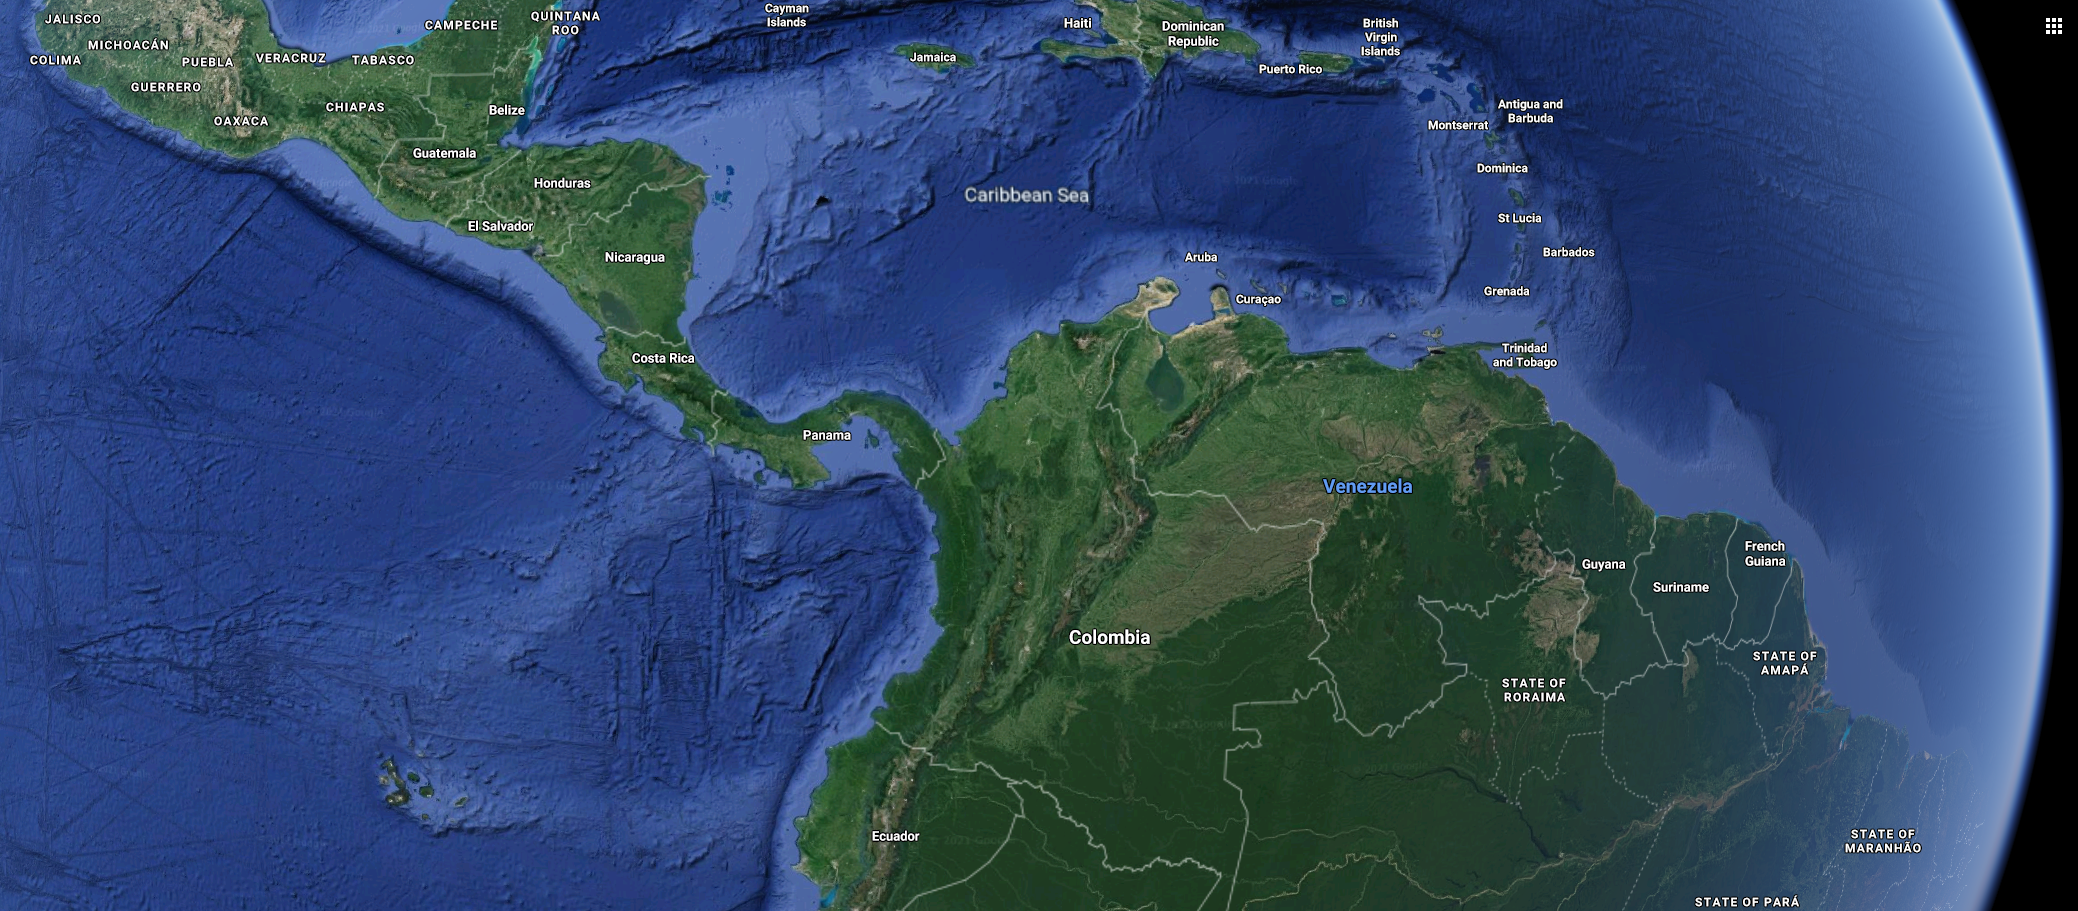
\includegraphics[width=10cm]{nueva_granada.png}
\caption{\label{fig:ng} A map of the Northern edge of South America and the Caribbean.}
\end{figure}

\begin{enumerate}
\item On Fig. \ref{fig:ng}, label the locations of the following cities:
\begin{itemize}
\item Quito
\item Santa Fe (de Bogot\'{a})
\item Caracas
\end{itemize}
\item List the universities in each of the above cities.  Which ones were founded with Enlightenment ideals in mind, and at which ones were taught concepts from Newtonian (as opposed Scholastic) physics? \\ \vspace{2cm}
\end{enumerate}

\section{Comparisons of Adoption of Scientific Revolution}

\begin{enumerate}
\item What do the contrasted examples of Jos\'{e} Ignacio Bartolache and Jos\'{e} Celestino Mutis say about the acceptance of the Scientific Revolution in the different \textit{virreinatos}? Give examples of the accomplishments of each person, and give context for the acceptance of the work of each in their respective \textit{virreinato}. \\ \vspace{3cm}
\item Discuss the educational roles of the Jesuits and the Dominicans in Nueva Granada\footnote{It might be helpful to know: Dominican universities were sometimes named \textit{San Tom\'{a}s}, after Saint Thomas Aquinas (not Saint Thomas the Apostle), because Saint Thomas Aquinas was a Dominican.  \textit{San Ignacio de Loyola} was the founder of the Jesuits, and some Jesuit universities are named \textit{San Ignacio}.}.  When did the Jesuits leave Nueva Granadan education, and why?  How did the Dominicans operate educational institutions as they asserted control over various universities? \\ \vspace{3cm}
\item Eventually, the Spanish Crown took control of education.  How did this happen, and more importantly, why would the Crown wish to do this?  Now turn your attention to the time before the Spanish Crown took over education.  \textbf{This one is worth a bonus point.}  \textit{How did control of education grant political control?  Why would the power to confer degrees give someone political power?} \\ \vspace{3cm}
\end{enumerate}

\section{Advent of Newtonian Physics in Nueva Granada}

\begin{enumerate}
\item Discuss the significance of the geodetic expedition of Charles de la Condamine in 1735.  What was the goal?  What were the cultural outcomes for Creole peoples, according to the writings of Alexander von Humboldt? \\ \vspace{1cm}
\item Which Catholic religious order first taught Newtonian physics in Nueva Granada?
\begin{itemize}
\item Carmelites
\item Dominicans
\item Franciscans
\item Jesuits
\end{itemize}
Did this order always teach Newtonian physics?
\end{enumerate}

\end{document}
